% Final Dissertation Report

%The document is a report
\documentclass[11pt,a4paper,oneside]{book}

%define horizontal rule
\newcommand{\HRule}{\rule{\linewidth}{0.5mm}}

\usepackage{fullpage}
\usepackage{pdfpages}
%use the listings package
\usepackage{listings}
%use the English language
\usepackage[english]{babel}
%use graphics
\usepackage{graphicx}
%use wrap figures
\usepackage{wrapfig}
%geometry stuffs
\usepackage{lscape}
%use captions
\usepackage{caption}
%use multi-row tables
\usepackage{multirow}
\usepackage{url}
\usepackage{breakurl}
\usepackage{subcaption}
\usepackage{rotating}
\usepackage{pdflscape}

\usepackage[nottoc,numbib]{tocbibind}

\usepackage{fancyhdr}
\setlength{\headheight}{15pt}

\pagestyle{fancy}



\begin{document}

%include the title page
\newcommand{\Revision}{678f948}

\begin{titlepage}
 
\begin{center}

% Upper part of the page

\includegraphics[width=0.20\textwidth]{../cover_logo.png}\\[1cm]


\textsc{\LARGE Aberystwyth University}\\[0.5cm]
\textsc{\LARGE Final Report}\\[0.5cm]



 
% Title
\HRule \\[0.4cm]
{ \huge \bfseries Partridge: An Intelligent Literature Analysis and
Recommendation Suite.}\\[0.4cm]

\HRule \\[1.5cm]

 % Author and student ID
\begin{minipage}{0.4\textwidth}
\begin{flushleft} \large
\emph{Author:}\\
\textsc{James Ravenscroft}\\
jrr9@aber.ac.uk\\
090407039\\
\end{flushleft}
\end{minipage}
\begin{minipage}{0.4\textwidth}
\begin{flushright} \large
\emph{Supervisors} \\
Amanda Clare (afc)\\
Maria Liakata (mal)

\end{flushright}
\end{minipage}


\vfill

\textsc{Submitted in partial fulfilment of requirements for a Batchelor of
Science Degree at Aberystwyth University}



\vfill
 
% Bottom of the page
\textsc{\large Word Count: 0}\\
\textsc{\large Status: Draft}\\
\textsc{\large Revision: \Revision{} }\\
{\large \today}
 
\end{center}

\frontmatter
 
\end{titlepage}



%some definitions for paragraph layout stuff
\setlength{\parindent}{0pt}
\setlength{\parskip}{1.5ex plus 0.5ex minus 0.2ex}



\thispagestyle{plain}

\begin{center}
\textsc{\large Statement of Originality}
\end{center}

This submission is my own work, except where clearly indicated.  

I understand that there are severe penalties for plagiarism and other unfair
practice, which can lead to loss of marks or even the withholding of a degree.
I have read the sections on unfair practice in the Students’ Examinations
Handbook and the relevant sections of the current Student Handbook of the
Department of Computer Science.  

I understand and agree to abide by the University’s regulations governing these
issues.\\\\

........................................

\pagebreak
\thispagestyle{plain}

\begin{center}
\textsc{\large Acknowledgements}
\end{center}

I would like to take this opportunity to thank both of my
supervisors, Dr Amanda Clare and Dr Maria Liakata, for giving up so much of their
time to support me in designing and developing this project. 

Thanks to the users who tested Partridge once it was made generally available
and for their feedback in the form of bug reports and suggestions. Especially
my close friends Alexander Brown and Douglas Eggleton who provided a great deal
of feedback throughout the project. I would also like to thank Matt Pugh for
helping me decide on the name of the project.

Finally, I am eternally grateful for the support of my family and friends who
have put up with my gripes and moans throughout the duration of this project
and, without whom, I couldn't have achieved such an ambitious project.

\begin{center}
\line(1,0){250}
\end{center}

The image on the front cover is an illustration of a Partridge, donated to the
public domain by Pearson Scott Foresman in 2007. A list of their donations can
be found at
\url{http://commons.wikimedia.org/wiki/Commons:Pearson_Scott_Foresman}

\pagebreak
\thispagestyle{plain}


\begin{center}
\textsc{\large Abstract}
\end{center}

When faced with the great number of scientific papers made general available on
the internet, it is often very difficult for researchers to find relevant
scientific literature. This project aimed to build an information retrieval and
recommendation tool that uses Natural Language Processing and Machine Learning
techniques to present the most relevant scientific papers to a user based upon
their search criteria and preferences.

A preprocessing system that exploits existing Natural Language Processing tools
was used to analyse a large sample of research papers, labelling the presence
of conceptual zones within each paper and extracting metadata.  Decision trees
were also trained to classify papers into well established type categories
based upon the relative proportions of the types of conceptual zones
present within the papers. 

A web interface was built to facilitate fine grain search, making use of the
zone information captured during preprocessing. Filtering of papers using their
type as determined by the preprocessor was also built in. Individual papers
returned during searches are presented in their own profile page that provides
charts and extra metadata to help researchers to understand the paper's
content. A page allowing authors and rightsholders to submit their own papers
for analysis was also created to allow the scientific community to extend the
impact and utility of the system.

The machine learning systems used within the project have been evaluated and
found to be accurate to 87.9\% when classifying a paper's type. The possibility
of extending the machine learning capabilities of the system to categorise
papers by subject domain and outcome of experimental results is discussed as
well as the potential for further improvements to the user interface.

A working version of the software has been made generally available at
\url{http://farnsworth.papro.org.uk} and can be explored and used by the
general public. It is hoped that over the coming months, the system will grow
to become a far reaching, widely used tool for academic research.


\tableofcontents

\pagebreak

\mainmatter

\chapter{Introduction}
%%%%------------------------------------------------
%
%  Include for chapter one of dissertation: introduction
%
%%%%------------------------------------------------
\subsection{Context}

\subsection{Background}

\subsection{Objectives}

\subsection{Literature Review}


\chapter{ Development Methodology }
Chosing an effective development methodology can play a very large part in the
success or failure of a software project. A number of existing development
methodologies have been developed and used very effectively over the last 50
years. However, custom methodologies are also commonly used for projects that
aren't suited to one of the commonly used approaches. Some common approaches to
software development and the formulation of a custom methodology for Partridge
are discussed below.

\section{Existing Methodologies} 

Under the traditional `Waterfall' Software Development model, Requirements
Gathering, Analysis, Program Design, Coding, Testing and Operations were all
defined as formal phases in the development cycle. There is little flexibility
other than moving back up the waterfall to rectify mistakes after
testing\cite{Royce:1987:MDL:41765.41801}. This model was very focused on
paperwork and bureaucracy, trying to maintain a paper trail and manage risk
through accountability \emph{(Ibed)}. This approach to software development is
very heavyweight and slow and often produced software that did not match the
users' needs as a result \cite{Boehm1988}.

As an alternative to the heavyweight Waterfall approach, Beck \emph{et al.}
came up with the principle of the Agile Manifesto, favouring a lightweight,
responsive development model over the heavyweight slow waterfall
system\cite{beck2001agile}. Many of Beck's ideas focus around working in a team
of developers and prioriting communication between team members \emph{(Ibid.)}.
This is most prominent in the Extreme Programming (XP) method of software
development. Since Partridge is an individual project, XP was not really
applicable. However, some concepts like rapid prototyping/spike work and
iterative release cycles were used as part of the Partridge development
methodology.

\section{ Partridge's Development Methodology}

A custom methodology was used for keeping track of development within
Partridge.  All design and planning documentation have been written up and
placed on a wiki which is accessible and modifiable by the author and both
supervisors. This creates a paper trail for all tasks and also allows
collaboration between involved parties through the Internet.

Throughout the project, weekly meetings were held with both project
supervisors. The notes from the preceeding week were analysed and each task
discussed in depth. New tasks were then noted down along with any observations
that should be documented. These were then uploaded to the wiki the following
day or earlier. Each party present at the meeting adds their own observations
to the notes page. This page is then reviewed at the next meeting.

Partridge made use of an agile, `iterative' development process. A working
version of the system was released at the end of each month. Tasks to be
undertaken in each iteration were stored in GitHub's issue manager program.
Priority was given to those tasks that provided the most value for the least
time investment. Test users were also allowed to submit bug reports to the
tracker system, and these were given priority if they were serious.

Programming tasks were added to the GitHub project tracker facility in the
same place as the Wiki was hosted. The `milestones' feature, which allows tasks
to be split into groups that must be completed by an arbitrary date, was used
to plan iterations and could be used to provide precise summaries of how the
project was progressing. In January, the project ran behind by a few weeks.
The time tracker explained that the project was precisely 17 days behind and
highlighted the set of tasks that needed to be completed to bring the project
back up to speed.

\subsection{ Initial Plan and Project Timeline }

During the early stages of the Partridge project, an initial system design was
drawn up and a set of tasks that covered the system's implementation were
formulated. These tasks were divided up into iterations and added to the
project planner on GitHub. Each task's dependencies were carefully considered
in order to prioritise tasks properly. The initial project plan can be seen in
Appendix \ref{sec:timeline}. 

\subsection{Support and Version Control Tools}

Partridge made heavy use of GitHub and the Git version control system. Git,
developed by Linus Torvalds, is a distributed Version Control System (VCS) that
offers many of the features of centralised VCSes such as Subversion and CVS.
However, unlike these centralised products, Git repositories are
self-contained, requiring no connection to a central server, with each copy of
the repository containing the complete project history. Copies of the
repositories are stored on the development machine, the production machine and
the GitHub server. This makes GIT more reliable than centralised repositories
since all code is accessible regardless of whether the repository hosted with
GitHub is online.

GitHub's hosted project management tools and wiki were used to store project
tasks, notes and metadata during development.

\section{Summary}

Having analysed some of the existing development methodologies and determined
that most of the common methodologies were not suitable for Partridge. A custom
methodology was formulated and support tools chosen. Task analysis was then
performed and a project timeline generated. With a timeline in place, the
initial design phase for Partridge and its subsystems could begin.


\chapter{Design}
%%-----------------------------------------------
%
% Include for design chapter of dissertation
%
%%----------------------------------------------

\subsection{ Process Model }

\subsection{ System Design }

\subsection{}


\chapter{Implementation}
%%------------------------------------------------------
%  
%  Implementation include for dissertation
%
%------------------------------------------------------


\subsection{Technical Challenges}

\subsubsection{ Sourcing Scientific Papers}
For Partridge to be a success, it is important to include a large variety of
different scientific papers in its corpus. Therefore, several sources of
scientific papers were explored and considered.

The most convenient and accessible source is the ART corpus that SAPIENTA was
trained with\cite{citeulike:11077287}. This corpus is already stored using the
CoreSC schema and has been pre-annotated. This means that Partridge would not
need to do any conversion or pre-processing on the papers. These scientific
papers are all chemistry papers. Therefore, more papers from other scientific
domains are needed to get a wider variety of topics and make Partridge useful
to as wide an audience as possible. 

The `mega-journals' PLOS ONE \url{http://www.plosone.org/} and arXiv
\url{http://www.arxiv.org/} were suggested as sources for more open access
articles that could be added to Partridge. Both of these sites were found to
contain large volumes of open access papers. However, most of these papers were
published as PDF files which meant that some conversion would be required to
make them compatible with Partridge.

\subsubsection{PDF Conversion}
Most scientific papers available on the internet are formatted as PDF
documents. However, Partridge uses and stores documents that use the CoreSC
schema by Soldatova and Liakata\cite{liakata2008guidelines}. Therefore some
spike work was carried out to determine the feasibility of converting papers
published as PDF documents into XML documents. Townsendi \emph{et al.} (2009) liken converting
PDF to XML to ``converting hamburgers into cows," they go on to explain that
PDF documents do not contain any semantic data and documents lose much of their
explicit structure when they are formatted in this way \cite{Townsend2009}.
Therefore, to convert PDF documents into an NLP-friendly format, some
heuristics must be used to detect the document's structure\cite{pdfminer}.

This was the first big challenge in the project. A prototype script was written
using a Python PDF extraction library called PDFMiner
(\url{http://www.unixuser.org/~euske/python/pdfminer/index.html}).  This
toolkit already contains some heuristics about how to extract text from PDF
documents, grouping together characters that appear very close to each other,
and separating paragraphs and headings when a larger area of whitespace is
detected\cite{pdfminer}. Despite these rules, the library still produced some
extraneous whitespace and newline characters as part of the output. A
subroutine to trim whitespace and newlines was added to the script to resolve
this problem. 

The next stage was to split the text into sentences in preparation for
processing with SAPIENTA. With the assistance of the NLTK library, a sentence
splitting subroutine was implemented. This used a machine learning algorithm
that had been trained to recognise sentence boundaries to split the text. Each
sentence was then added to a CoreSC compatible XML document for processing by
SAPIENTA.

Initially, the PDF conversion subroutine had a very high error rate due to the
variation in the formatting of scientific papers. It was suggested that PDFX
(\url{http://pdfx.cs.man.ac.uk/}), a free service hosted by the University of
Manchester could be used instead of PDFMiner for the initial PDF data
extraction. The main advantage of PDFX over the PDFMiner library is that it is a
trained machine learning system that has been trained using a large full-text
selection of scientific articles; PDFMiner uses more general heuristics
designed to process a large selection of different types of PDF document.

PDFX also provides output that already has some metadata, such as title,
author, and abstract, associated with it. PDFMiner did not provide any
metadata, and it was necessary for the script to guess which passage of text
was the abstract after the initial text extraction stage.

With the new PDF extraction method in place, the script ran without the need
to modify either of the whitespace sanitiser or sentence splitter routines. The
process was much more successful and able to produce SAPIENTA-compatible
documents from most of the PDF input files that were provided.

\subsubsection{Pre-processing with SAPIENTA}

With a successful PDF conversion script, the next step was to try and run
SAPIENTA over the converted papers and annotate them, ready for inclusion in
the Partridge corpus.

By default, SAPIENTA is packaged as a web-based tool, written in Java, that
can be downloaded (from \url{http://www.sapientaproject.com/software}) and used
to annotate one paper at a time. Dr Liakata was able to provide information on
two alternative ways of using the system. One method was to submit a remote
procedure call (RPC) to a server running SAPIENTA with a batch of papers and
retrieve the output. The other method was to use an alternative version of the
code that runs locally in a Python environment and could be modified to process
papers as a batch.

A script was written to send un-annotated XML documents to the remote SAPIENTA
server and retrieve a list of annotations. This worked well until the server
stopped replying to requests. This meant that no further conversions could be
carried out until the server was repaired and raised concerns about how the
remote servers might cope with a large number of automated requests from a
full version of Partridge.

The Python version of SAPIENTA was then downloaded and a test executed.
Unfortunately there were several data files missing from the package that had
to be acquired from Dr Liakata. 

SAPIENTA for Python also relies upon a package called CRFSuite which implements
Conditional Random Fields, a method for segmenting and labelling sequence
data\cite{CRFsuite}. This library did not compile properly on the test
environment and its creator had to be contacted via a mailing list (See
Appendix \ref{sec:crfemail}. After a few days, the owner responded and the
library was compiled successfully.  

Once all the data files and libraries were successfully in place, the Python
version of SAPIENTA was used to process some of the papers converted from PDF.
This was a great success and the annotations provided by SAPIENTA seemed to be
accurate. 



\chapter{Testing}
\label{chapter:testing}
%%------------------------------------------------------
%  
%  Testing include for dissertation
%
%------------------------------------------------------

\subsection{ Unit Testing }


\subsection{ User Testing } 

Once a basic user interface had been implemented, the system was opened for
user testing. The main Patridge instance
(\url{http://farnsworth.papro.org.uk/}) was advertised using several social
media streams and users encouraged to submit bug reports if they experienced
any problems whilst using the site.


\subsection{ Testing Learning Algorithms }

Patridge uses machine learning algorithms to classify the type of research
papers added to its database. It was therefore necessary to test that these
algorithms were sufficiently trained and provide accurate classification.
Unlike 


\chapter{Critical Evaluation}
%%------------------------------------------------------
%  
%  Evaluation include for dissertation
%
%------------------------------------------------------

\subsection{ Achievements }

\subsection{ Limitations and Potential Improvements }

\subsection{ Further Research }


\pagebreak
\bibliographystyle{IEEEannot}
\bibliography{report}

\appendix

\appendix
\section{User Interface Designs}
\label{sec:ui_designs}

\subsection{ Partridge Query Interface}


Figure \ref{fig:ui_mockup} shows the user interface that will be utilised to
search and query Partridge's corpus. 

The query form shows two main sections: Filters and Keywords. 

Filters can be used to show a large set of papers where the user is unsure of
what to search for. Users will be able to look for papers by type and topic as
discussed above. The paper result filter has not been included in this diagram.
However, it is expected that a drop down menu for result type would be included
in the filters section of the form.

Keywords allows the user to look for a set of keywords that is specifically
within a CoreSC concept for a paper. For example, the reader may want to find
experiments that use a server farm to do lots of calculations. Therefore, they
would enter ``Server Farm" as their keywords and chose ``Method" from the paper
section. The user then adds this to the set of keyword queries in the table
below the text field with the add button.

Once a user has configured both filters and keywords to their preferences, they
click the search form to run the search itself.

Other notable features on this mockup include a list of most recent searches.
This helps the user to understand how to use Partridge and gives them some
suggestions for what they might search for. Similar listings are provided for
the most popular papers in the Partridge database and the most recent papers
added to the system.

\begin{figure}[!ht]
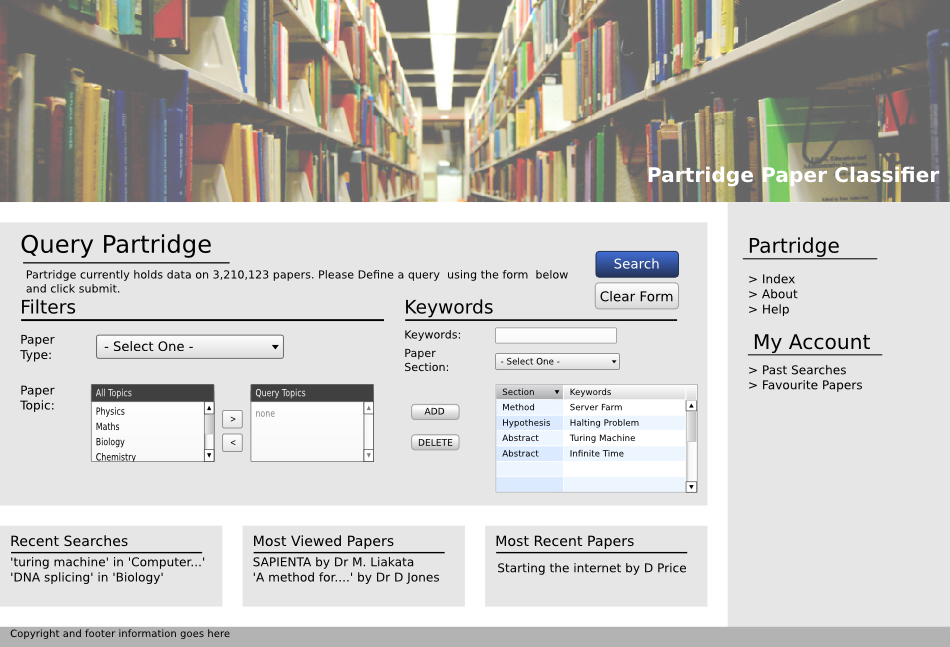
\includegraphics[width=\textwidth]{images/mockup_1.png}
\caption{User interface design for querying Partridge}
\label{fig:ui_mockup}
\end{figure}


\section{System Process Diagrams}
\label{sec:system_diagrams}

This section documents the system process diagrams that have been produced. The
first completed diagram shows how a paper will be added to Partridge and the
actions that will be carried out upon it.

\subsection{Adding a Paper to Partridge}

\begin{figure}[!ht]
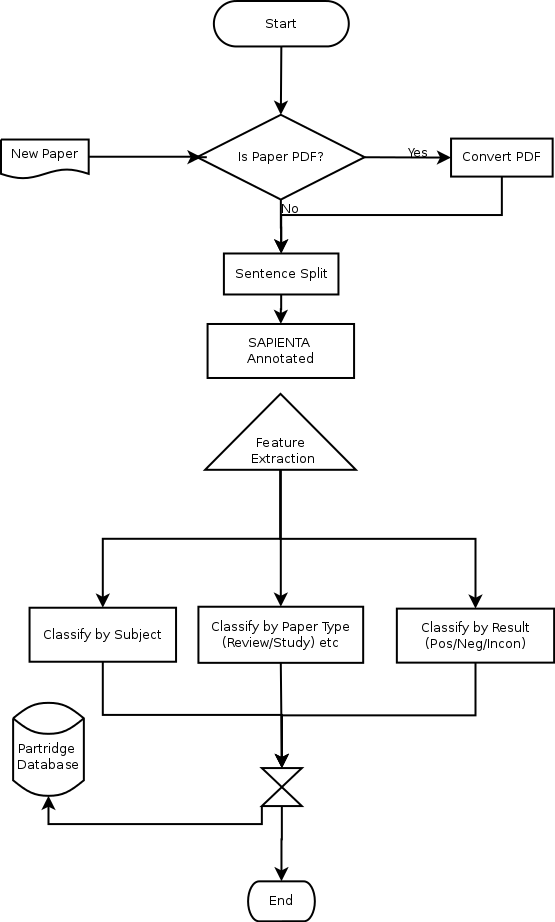
\includegraphics[width=0.75\textwidth]{images/PaperAddedProcess.png}
\caption{The process of adding a new paper to Partridge}
\end{figure}

The system starts off by converting the document to XML from PDF if necessary
through the use of the PDFX tool provided by Manchester University. A sentence
splitting tool is then used to parse the resulting document and separate the
sentences.

Once the sentences have been split, Maria's SAPIENTA tool is used to annotate
each sentence to determine which of the core scientific concepts it covers.
This information is stored back in the XML file with the document.

After this, feature extraction is carried out upon the document to find useful
features for the following classification tasks:

\begin{enumerate}
\item Paper topic/subject -i.e. is the paper a biology paper or a computer science paper?
\item Type of paper - i.e. is the paper a case study, an experiment or a literature review?
\item Paper result - i.e. did the paper have a positive, negative or inconclusive result?
\end{enumerate}

These classifiers are then run (they could potentially be run in parallel if
processing power is available) to determine the paper's class for each
classifier respectively. The data gathered along with any paper metadata
captured such as title, author, date, institute etc are then stored in the
database.


\section{Email for CRFSuite}
\label{sec:crfemail}
\begin{verbatim}
Hi All,

I'm trying to build CRFSuite's python extension 
(http://www.chokkan.org/software/crfsuite/) on an Arch Linux 64-bit 
environment using Swig 2.0.8 (PCRE enabled).

When I run SWIG, I get the following output:

<<OUTPUT OMITTED FOR BREVITY>>

Full output available at http://sourceforge.net/mailarchive/message.php?msg_id=30024209

As far as I can see, all of these problems stem from this declaration in 
the SWIG input file (http://pastebin.com/9JipJ1C1):
%template(ItemSequence) std::vector<CRFSuite::Item>;

I've had a look around on google and on this mailing list and the only 
other "cannot copy typemap" errors I've encountered have been where 
people have excluded the std namespace in favour of a 'using' statement. 
As you can see, this example uses absolute class names so that isn't the 
issue here. I haven't had any luck contacting the software maintainer 
for CRFSuite yet either.

As you might expect, if I continue to compile the extension without 
heeding these errors, when I try to make use of the ItemSequence object 
I get the following python error:
TypeError: in method 'ItemSequence_append', argument 2 of type 
'std::vector< CRFSuite::Item >::value_type const &'

I'm going to keep trying to sort this out and if I find the solution 
independantly, I'll make sure to post a follow-up email. However, if 
anyone else has any ideas about what might be happening here, please let 
me know.

Thanks,

James Ravenscroft
AI & Robotics Undergraduate
Aberystwyth University
\end{verbatim}


\section{Project Timeline}
\label{sec:timeline}

This table shows the projected timeline for the Partridge project. These
calculations were carried out under the assumption of 2 full days of work per
week on the project and one iteration equating to one month (28 days). There
will be 7 iterations in total and after each, a new version of Partridge will
be made available (except for iteration zero which is a research only
iteration).


\begin{figure}[htp] 
 \vspace{ -1cm }
 \centering{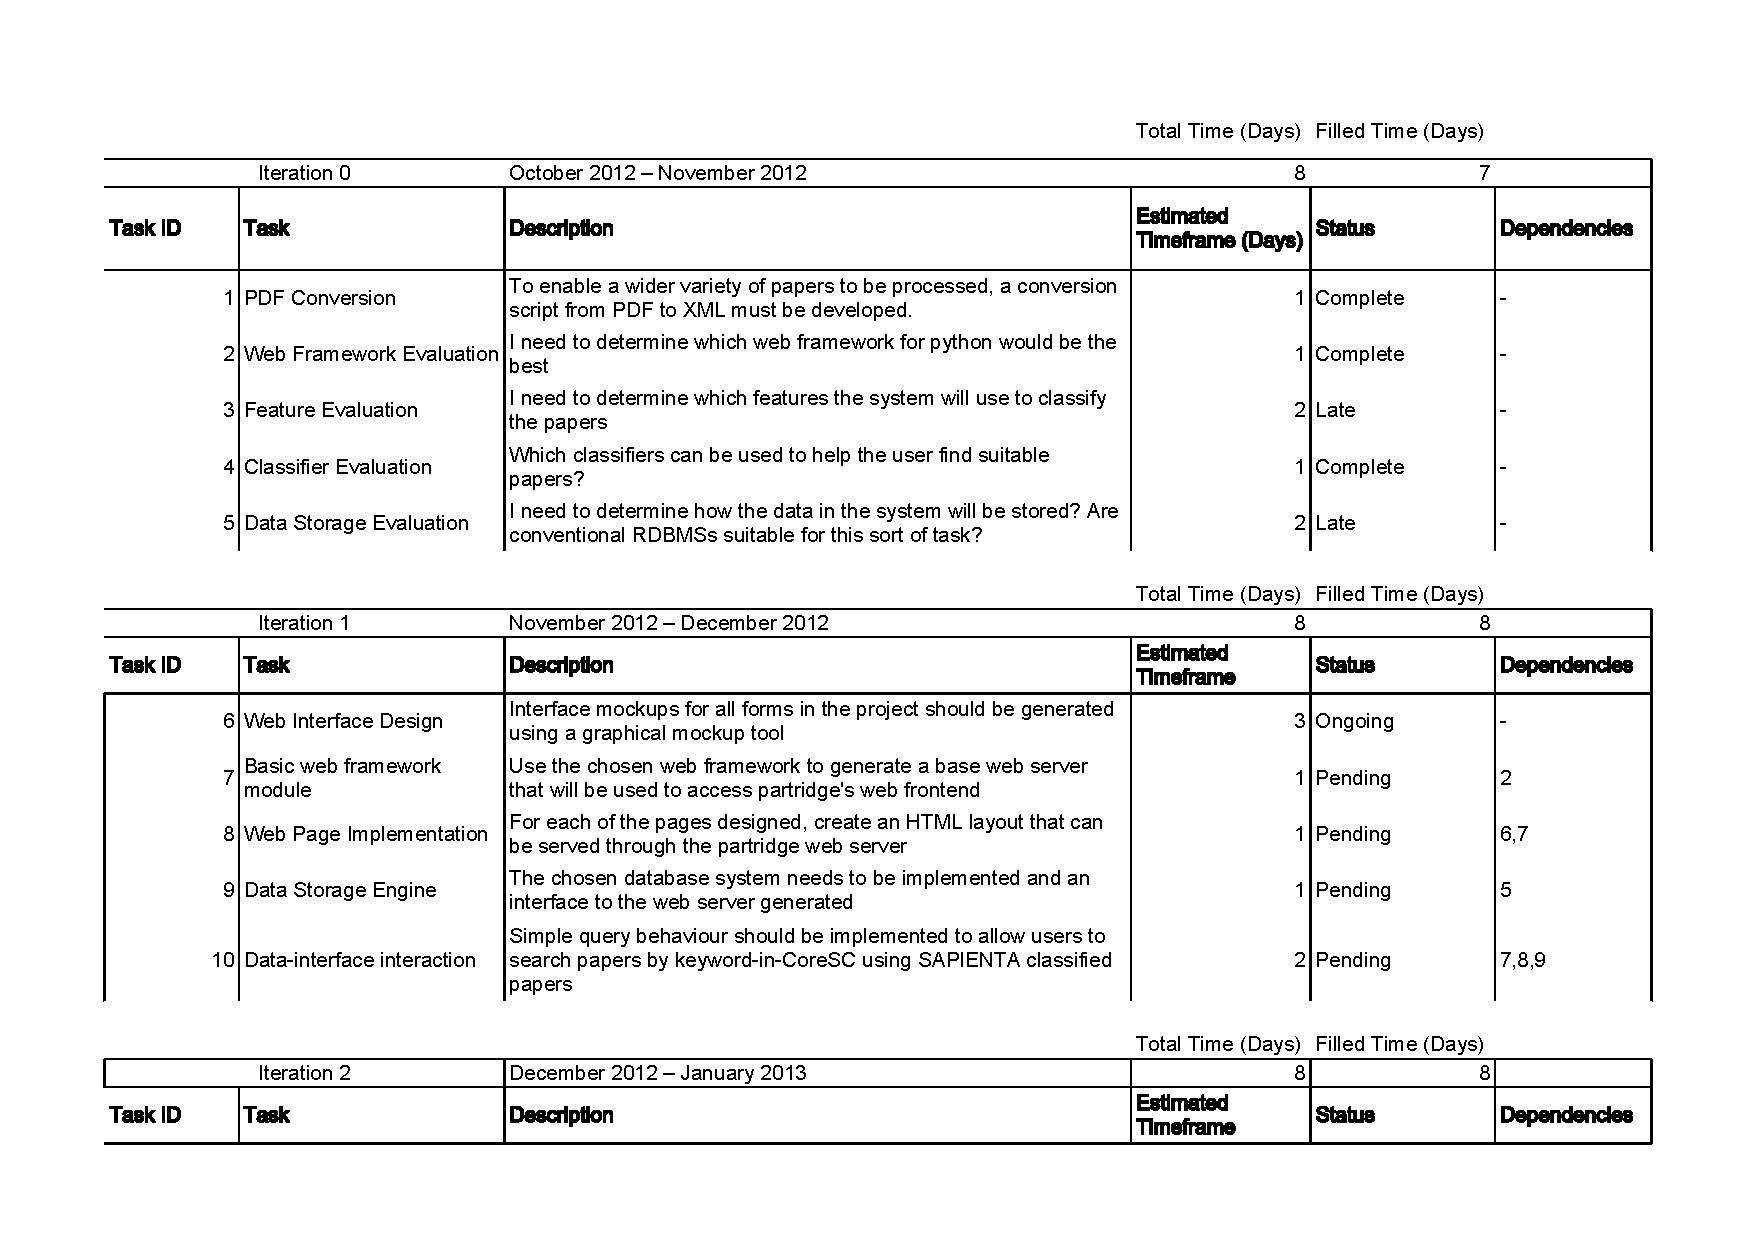
\includegraphics[scale=0.60,page=1]{../timeline.pdf}}
  
\end{figure}

\begin{figure}[!htp] 
 \centering{\includegraphics[scale=0.60,page=2]{../timeline.pdf}}
 \vspace{-2cm}
\centering{\includegraphics[scale=0.60,page=3]{../timeline.pdf}}
\end{figure}

\pagebreak
\section{Project Wiki}
\label{sec:wiki}

All pages from the Wiki are shown below with the exceptions of those pages
which have already been mostly featured in the document (UI Mockups and
Progress Diagrams and the project timetable are not shown in this section).

\subsection{ Notes 03/10/2012 }
\subsection{Meeting Notes from 03/10/2012}

\subsubsection{General topics}

\begin{itemize}
\item
  Talked about using research papers instead of books :-
\item
  copyright issues - mainly resolved because of Gutenburg project
\item
  processing issues - too much information to process quickly and
  realistically
\item
  Maria has some software for identifying sections in papers - could be
  used to help locate specific features
\item
  There are quite a few sources for papers that could be used for the
  project:
\item
  http://arxiv.org/
\item
  http://plosone.org/
\item
  Maria's papers are in XML format
\item
  Formatting may or may not be an issue - PDFs are a nightmare to parse
\end{itemize}

\subsubsection{Things to consider}

\begin{itemize}
\item
  What sort of recommendations for different sources might there be and
  how would these recommendations be extracted?
\item
  Feature engineering - what sorts of features might there be to pick
  out in the papers?
\item
  I need to have a read through the sentiment analysis paper that Maria
  has been working on
\item
  I need to have a play with the software for identifying sections in
  papers.
\end{itemize}

\subsubsection{Misc concerns}

\begin{itemize}
\item
  Decided that our weekly meeting should be Wednesdays at 3pm
\item
  Investigate setting up source control and a wiki (that's been done as
  you can tell)
\end{itemize}


\subsection{ Notes 10/10/2012 }
\subsection{Meeting Summary 10/10/2012}

\subsubsection{From Maria's notes}

\begin{itemize}
\item
  James has gone through papers and thinks would be more doable to work
  with papers than Books
\item
  James has found the XML format of PlosOne and ART/CoreSC corpus
\item
  Domain needs to be determined
\item
  Maria to send paper on sentiment analysis of citations
\end{itemize}

\subsubsection{Current features and recommendations}

\begin{itemize}
\item
  Analysis of results section - positive or negative result
\item
  Potentially look at writing styles of authors using syntactic analysis
\item
  Isolating terms within sections of papers (i.e.~find me papers where
  methodology x was used)
\item
  finer grain analysis of CoreSC categories
\item
  nltk python toolkit. What other toolkits? Would jerboa be any good?
\item
  common features for sentiment analysis
\end{itemize}

\subsubsection{Basic system design}

I have started a basic system design although it is very basic at the
moment. [Image Omitted]

\subsubsection{Background - Similar Systems and how they work}

\begin{itemize}
\item
  Google Scholar
\item
  Mendeley
\item
  Citeulike
\item
  Tweeting or `liking' on facebook.
\end{itemize}

\subsubsection{Reading}

\begin{itemize}
\item
  TF-IDF
\item
  Take a brief look at journal of negative results
\item
  `Bigrams + trigrams' and syntactic pattern finding
\item
  Common features used in NLP
\item
  Sentiment analysis of citations in papers
\item
  `Bag of words'
\end{itemize}

\subsubsection{Coding/practical research}

\begin{itemize}
\item
  Play some more with SAPIENTA
\item
  Implement a (La)TeX to SciXML or pubmed command-line tool.
\end{itemize}


\subsection{ Notes 19/10/2012 }
\subsection{Notes from Meeting 18/10/2012}

\subsubsection{General Comments}

\begin{itemize}
\item
  I need to decide on a domain for the project. It may be that papers on
  a varied selection of topics would be a good start
\item
  Decided on an agile development cycle with a basic program that is
  improved in `iterations'.
\item
  As part of testing the software, it may be possible to get other final
  year students to trial the engine and use it to make recommendations
  for their reading.
\item
  I need to investigate ways of analysing papers for syntactic patterns.
  This may be indicative of:

  \begin{itemize}
  \item
    Different authors' writing styles
  \item
    Different types of paper -i.e.~psychology vs physics
  \end{itemize}
\end{itemize}

\subsubsection{TODO}

\begin{itemize}
\item
  Revisit PDF to XML conversion as conversion from PDF would make life a
  lot easier
\item
  Maria mentioned that she may have access to an HTML to XML program
  which would be good to look at.
\item
  Check out python Jerboa to see if it would be useful for the project.
\end{itemize}


\subsection{ Notes 24/10/2012 }
\subsection{Notes from meeting 24/10/2012}

Amanda was not present for this meeting.

\subsection{Discussed}

\begin{itemize}
\item
  We discussed the PDF conversion routine and decided that whilst
  important, it is crucial not to get too caught up in this.
\item
  Maria is going to send me a link to an existing PDF to XML converter
  that might provide the functionality with some tweaking - or at least
  help
\item
  We discussed the Python version of Sapienta which currently supports
  SciXML and simplified versions thereof.
\item
  Maria needs to send me a couple of data files for this to work
  properly.
\item
  Confirmed that Jerboa is a Java library (I was confused because I was
  expecting a python toolkit) and need to look at it properly now.
\item
  Discussed the actual functionality of the system and came up with a
  brief system outline, around which I can plan.
\end{itemize}

\subsection{TODO}

\begin{itemize}
\item
  Now that we know what the system is going to do (See System Outline), I need to look at features that
  will allow us to:
\item
  Pre-classify documents based on their topic, type, result etc
\item
  Determine document similarity based on user preference from their
  tagging etc. (I can make use of the ``Features in sentiment analysis''
  paper for this)
\item
  Run more tests on the PDF parser and potentially look at another
  solution if this takes up too much time.
\item
  Have a go with Python SAPIENTA once the data models are present
\end{itemize}


\subsection{ Notes 31/10/2012 }
\subsection{James' Meeting Notes}

\subsubsection{To Think about}

\begin{itemize}
\item
  Discussed imminent deadline for project progress report - 19/11/2012
\item
  Decided that having a report finished by 14/11/2012 would be a good
  report to give Amanda and Maria a chance to check over the report
  before handin.
\item
  Maria explained that it is possible to send a batch of papers to
  Sapienta rather than one at a time. She is going to provide
  information on how this can be achieved at some point during the week.
\item
  I should describe my working processes and why they are helpful.
\end{itemize}

\subsubsection{Todo}

\begin{itemize}
\item
  We discussed the merits of using the pdfx converter instead of my
  script - might have plug-and-play compatibility with Sapienta for a
  start - need to verify this.
\item
  I need to send my error message the CRFSuite compilation to Maria so
  that she can contact the maintainer.
\item
  I need to expand on the system outline providing more specific goals
  and timeframes - this will become my development plan.
\item
  I need to look at textpresso and see if it will help me with my
  comparison/evaluation
\end{itemize}


\subsection{ Notes 07/11/2012 }
\subsection{Notes from 7/11/2012}

\subsubsection{Discussed}

\begin{itemize}
\item
  What I'll need to have for my demo:

  \begin{itemize}
  \item
    Simple web interface
  \item
    Few basic classifiers - probably result of paper positive/negative
    and maybe paper type - proportions of coreSC concepts.
  \item
    Could show off PDF to XML converter script
  \end{itemize}
\end{itemize}

\subsubsection{To Consider}

\begin{itemize}
\item
  Is the disparity between bio paper CoreSC classification and other
  sorts of paper to do with Sapienta's model or does it demonstrate a
  feature - different subjects may have different proportions of each
  concept.
\item
  If I'm using distribution of concepts as an aggregate feature, I need
  to make sure the system does not fall over if a concept is missing.
\item
  Front end interface:
\item
  Need to find a new word for `section' Scientific Concept may be a bit
  too `scary', is there a better term for this?
\item
  If I allow users to upload papers, they must sign a digital disclaimer
  to say that they have the right to do so
\item
  There should be a ``report copyrighted material'' system
\end{itemize}

\subsubsection{To Do}

\begin{itemize}
\item
  Biggest task this week: Progress Report.

  \begin{itemize}
  \item
    Draft due 14/11/2012 for discussion on 15/11/2012
  \item
    Final deadline 19/11/2012
  \item
    Could provide wiki content as an appendix to the report
  \item
    Come up with a project timeline - actually consider dates
  \item
    Start with the web interface and work upwards.
  \end{itemize}
\item
  Send Maria the missing header file from crfsuite
\item
  Link system outline from wiki index
\item
  Maria said she'd look for a topic detection paper for me to peruse
\item
  I need to have another look at relevant features - struggling with
  this
\item
  Make a wiki list of features that could be used for classification
\end{itemize}




\pagebreak
\bibliographystyle{IEEEannot}
\bibliography{report}


\end{document}
